% *******************************************************************************
% * Copyright (c) 2007 by Elexis
% * All rights reserved. This document and the accompanying materials
% * are made available under the terms of the Eclipse Public License v1.0
% * which accompanies this distribution, and is available at
% * http://www.eclipse.org/legal/epl-v10.html
% *
% * Contributors:
% *    G. Weirich - initial implementation
% *
% *  $Id: einleitung.tex 4904 2009-01-03 17:58:33Z rgw_ch $
% *******************************************************************************
% !Mode:: "TeX:UTF-8" (encoding info for WinEdt)

\section{Introduction}
Pour établir des lettres , ordonnances, certificats etc. Elexis utilise de façon standardisée un logiciel valable : OpenOffice
Ceci ne doit pas forcément être la seule solution car le traitement de texte est appliqué par Elexis en forme de Plugin. On pourrait donc aussi laisser créer un Plugin pour Microsoft\texttrademark{}Office\texttrademark{}  ou n'importe quel autre logiciel de traitement de texte. Nous nous limitons ici par contre à l'OpenOffice qui est le logiciel de référence pour Elexis.
L'origine de OpenOffice se trouve dans StarOffice qui avait été développé dans les années 80 et qui représente aujourd'hui une Office-Suite en analogie à Microsoft Office avec la différence qu'il s'agit d'un produit open source disponible pour plusieurs systèmes d'exploitation.
Dans l'installateur de la version Windows de Elexis une version adaptée de OpenOffice.org est intégrée. Sous Linux on peut se servir de la version OpenOffice qui est normalement intégrée dans Linux. Pour Macintosh l'intégration ne fonctionne malheureusement pas encore. Faites attention de n'installer q'une seule version de OpenOffice sur votre système car sinon ceci pourrait provoquer des conflits entre les versions.


\medskip

Après l'installation de OpenOffice et de Elexis il faut que les deux programmes 'fassent connaissance'. Pour ceci il faut configurer le Plugin de texte dans Elexis de sorte qu'il ait accès sur OpenOffice.(Le Plugin
\glqq NOA-Text\footnote{Nous utilisons le module 'Nice Office Access' de \href{http://www.ubion.org}{www.ubion.org}
 pour intégrer OpenOffice}\grqq{}doit être installé, chose qui est normalement d'emblée le cas.

Séléctionnez dans le menu  \textsc{Fichier - Options} Vous trouvez dans la liste à gauche : \textsc{Traitement de texte}
Il y apparaît un boite de dialogue comme en \ref{fig:text1}. Choisissez là  \glqq
%\usepackage{graphics} is needed for \includegraphics
\begin{figure}[htp]
\begin{center}
  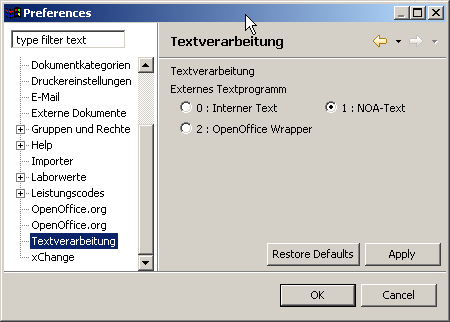
\includegraphics{images/text1}
  \caption{Konfiguration des Textplugins}
  \label{fig:text1}
\end{center}
\end{figure}

NOA-Text\grqq{}. Après vous choisissez dans la liste à gauche OpenOffice.org (cf Fig. \ref{fig:text2}
En cliquant sur \glqq définir\grqq{} vous définissez le chemin d'accès à votre installation OpenOffice.
%\usepackage{graphics} is needed for \includegraphics
\begin{figure}[htp]
\begin{center}
  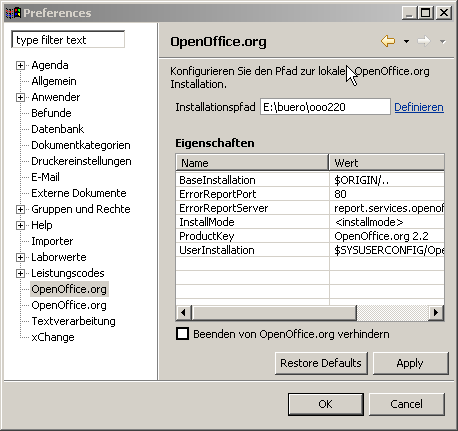
\includegraphics{images/text2}
  \caption{Konfiguration der OpenOffice-Installation}
  \label{fig:text2}
\end{center}
\end{figure}
Vous cliquez ensuite dans la boite de dialogue qui s'ouvre sur OpenOffice.org et cliquez sur 'terminer'.
Dans la boite de dialogue encore ouverte vous cliquez sur 'ok'. OpenOffice devrait être à disposition dès le prochain démarrage de Elexis. Lors de la première utilisation vous devez encore accepter les conditions de licence de OpenOffice.org.)



